\documentclass[12pt,a4paper]{article}

% ── Packages ─────────────────────────────────────────────────────────────────
\usepackage[margin=2.5cm]{geometry}
\usepackage{amsmath,amssymb}
\usepackage{graphicx}
\usepackage{booktabs}
\usepackage{hyperref}
\usepackage{cite}
\usepackage{setspace}
\usepackage{caption}
\usepackage{subcaption}
\usepackage{xcolor}
\usepackage{listings}
\usepackage{parskip}
\usepackage{titlesec}
\usepackage{abstract}

\hypersetup{
  colorlinks=true,
  linkcolor=blue!70!black,
  citecolor=blue!70!black,
  urlcolor=blue!70!black
}

\lstset{
  basicstyle=\small\ttfamily,
  breaklines=true,
  frame=single,
  backgroundcolor=\color{gray!10},
  language=Python
}

\onehalfspacing

% ── Title ─────────────────────────────────────────────────────────────────────
\title{\textbf{Self-Organised Criticality in the\\
               Drossel--Schwabl Forest Fire Model:\\
               Avalanche Dynamics and Connectivity}}

\author{Rayeli Nandy \\
 \small 2021CH70446\\
  \small Department of Chemical Engineering\\
  \small IIT Delhi
}

\date{April 10, 2026}

% ─────────────────────────────────────────────────────────────────────────────

\begin{document}
\maketitle

% ── Abstract ──────────────────────────────────────────────────────────────────
\begin{abstract}
\noindent
We investigate self-organised criticality (SOC) in the Drossel--Schwabl
forest-fire model using two-dimensional cellular-automaton simulations.
The model captures the three hallmarks of complex systems: stochastic noise
(lightning), cascading avalanches (fire propagation through connected tree
clusters), and spatial connectivity (tree density).
Starting from arbitrary initial conditions, the system spontaneously evolves
to a stationary critical state characterised by a broad distribution of
avalanche sizes.
Our simulations on an $80\times80$ lattice reveal a heavy-tailed avalanche
size distribution consistent with a power law $N(s)\propto s^{-\alpha}$,
with an estimated exponent $\alpha\approx0.44$, and demonstrate that
the mean avalanche size and frequency depend sensitively on tree density
(connectivity).
The critical density is maintained without external tuning, confirming
self-organised criticality.
These results are discussed in the context of real forest-fire ecology,
earthquake statistics, and other natural phenomena that exhibit scale-free
behaviour.
\end{abstract}

\textbf{Keywords:} self-organised criticality; forest-fire model;
avalanche; power law; cellular automaton; complexity science

\vspace{1em}
\hrule
\vspace{1.5em}

\clearpage
% ── 1. Introduction ───────────────────────────────────────────────────────────
\section{Introduction}

Many natural systems display catastrophic events whose size distribution
follows a power law over many orders of magnitude.
Earthquakes obey the Gutenberg--Richter law, stock-market crashes cluster in
time, neural avalanches in the brain span all scales, and forest fires burn
areas ranging from a single tree to entire landscapes \cite{Bak1987,Jensen1998}.
This ubiquitous scale-free behaviour is the hallmark of \emph{self-organised
criticality} (SOC), a concept introduced by Bak, Tang, and Wiesenfeld (BTW)
in 1987 \cite{Bak1987}.

In an SOC system, no external parameter needs to be fine-tuned.
The system \emph{drives itself} to the boundary between order and disorder---the
critical state---through the interplay of slow energy input and fast
dissipative relaxation.
At criticality, perturbations of all sizes (``avalanches'') occur with
frequencies governed by a power law, implying that the system has no
characteristic scale.

The forest-fire model of Drossel and Schwabl \cite{Drossel1992} is a paradigmatic
SOC cellular automaton.
Trees grow slowly on a two-dimensional lattice (slow drive, mimicking sunlight
and water), and are occasionally ignited by lightning.
A lit tree ignites its neighbours, so an entire connected forest cluster
burns in a single cascade.
The interplay of local connectivity (tree density) and stochastic ignition
naturally produces critical dynamics without parameter tuning.

The forest-fire model is an excellent candidate for studying complexity science
for several reasons.
First, it is directly motivated by a real ecological system with measurable
data.
Second, it cleanly separates the three components central to SOC: noise,
avalanche, and connectivity.
Third, its cellular-automaton structure admits efficient computer simulation
and transparent analysis.
Finally, the model is known to exhibit robust power-law behaviour whose
exponent has been studied analytically and numerically \cite{Christensen1993,Pruessner2004}.

The remainder of this paper is organised as follows.
Section~\ref{sec:model} describes the model, identifying its noise, avalanche,
and connectivity components.
Section~\ref{sec:simulation} details the simulation methodology.
Section~\ref{sec:results} presents the results.
Section~\ref{sec:discussion} discusses self-organised criticality and its
implications.
Section~\ref{sec:conclusion} concludes.

\clearpage
% ── 2. Model Description ──────────────────────────────────────────────────────
\section{Model Description}
\label{sec:model}

\subsection{Drossel--Schwabl Forest-Fire Model}

The model is defined on an $L\times L$ square lattice with periodic boundary
conditions.
Each cell $i$ can be in one of two states:
$\sigma_i \in \{\text{EMPTY}(0),\,\text{TREE}(1)\}$.
At each discrete time step the following rules are applied synchronously:

\begin{enumerate}
  \item \textbf{Lightning (noise):} Each TREE cell is struck by lightning
        independently with probability $f$. The fire then spreads
        \emph{instantaneously} to the entire connected cluster of trees
        (the 4-neighbour von Neumann neighbourhood) containing that cell.
        All trees in the cluster become EMPTY.
  \item \textbf{Growth (slow drive):} Each EMPTY cell independently becomes
        a TREE with probability $p$.
\end{enumerate}

The model is governed by a single dimensionless parameter,
$\theta = f/p$, which controls the ratio of ignition to growth rates.
For SOC behaviour we require $\theta \ll 1$ so that trees have time to form
large connected clusters before they are struck.

\subsection{Noise}

In the context of complexity science, \emph{noise} is the stochastic external
perturbation that drives the system.
In this model, noise is the lightning strike: a spatially random, temporally
Poissonian event that injects energy (ignition) into the system with
probability $f$ per tree per time step.
The noise is weak ($f=0.001$) relative to the recovery rate ($p=0.05$),
ensuring the system is driven slowly and has time to organise before the next
large event.

\subsection{Avalanche}

An \emph{avalanche} is a cascade event triggered by a single lightning strike.
When a tree at site $(r_0, c_0)$ is struck, the fire propagates to all
trees connected to it through a path of nearest-neighbour tree cells.
Formally, the avalanche is the connected component of the tree lattice
containing $(r_0, c_0)$, identified by breadth-first search (BFS).
The \emph{avalanche size} $s$ is the number of trees burned.

Avalanches range from $s=1$ (an isolated tree) to $s=L^2$ (the entire grid),
with the distribution of sizes being the central observable of interest.

\subsection{Connectivity}

\emph{Connectivity} is the degree to which trees are spatially linked.
It is measured by the mean tree density $\rho = N_{\text{tree}}/L^2$, which
controls the probability that a struck tree belongs to a large percolating
cluster.
Near the percolation threshold ($\rho_c \approx 0.59$ for the 2-D square
lattice), the cluster-size distribution itself follows a power law, so the
forest-fire model exploits percolation criticality as the mechanism for SOC.

The coupling between connectivity and avalanche size is central: higher $\rho$
means larger clusters and larger potential avalanches, while large fires
reduce $\rho$, providing the negative feedback that stabilises the system
near criticality without external tuning.

\clearpage
% ── 3. Simulation ─────────────────────────────────────────────────────────────
\section{Simulation Methodology}
\label{sec:simulation}

\subsection{Implementation}

The simulation was implemented in Python~3 using \texttt{NumPy} for vectorised
array operations, \texttt{Matplotlib} for visualisation, and \texttt{SciPy}
for statistical analysis.
The connected-cluster identification uses BFS via Python's \texttt{collections.deque}.
All code is available at \texttt{[GitHub repository URL]}.

\subsection{Parameters}

The main simulation used the parameters listed in Table~\ref{tab:params}.
The ratio $\theta=f/p=0.02$ ensures slow driving.
A burn-in period of 2000 steps was discarded before recording statistics to
allow the system to reach its stationary critical state.

\begin{table}[h]
\centering
\caption{Simulation parameters for the main run.}
\label{tab:params}
\begin{tabular}{lll}
\toprule
Parameter & Symbol & Value \\
\midrule
Grid size           & $L$    & 80   \\
Tree-growth prob.   & $p$    & 0.05 \\
Lightning prob.     & $f$    & 0.001 \\
Drive ratio         & $\theta=f/p$ & 0.02 \\
Burn-in steps       & ---    & 2000 \\
Production steps    & ---    & 8000 \\
Random seed         & ---    & 42   \\
\bottomrule
\end{tabular}
\end{table}

\subsection{Connectivity Sweep}

To study the dependence of avalanche statistics on connectivity, a second
set of simulations was performed on an $L=60$ grid with fixed $p=0.05$ and
$f$ varied from $0.0002$ to $0.02$.
For each value of $f$, the steady-state tree density $\rho$ (connectivity)
and avalanche statistics were recorded after a burn-in of 1000 steps.

\subsection{Power-Law Fitting}

The avalanche size distribution was binned on a logarithmic scale.
A linear regression was applied in log-log space to estimate the power-law
exponent $\alpha$ and the coefficient of determination $R^2$.
Only bins with count $>3$ were included in the fit to avoid noise at the
tails.

\clearpage
% ── 4. Results ────────────────────────────────────────────────────────────────
\section{Results}
\label{sec:results}

\subsection{Spatial Structure}

Figure~\ref{fig:snapshots} shows three snapshots of the forest grid at
different times.
At early times (immediately after burn-in), the grid shows a patchy landscape
with no dominant spatial scale.
By mid-simulation and into the late (stationary) state, the system develops
a characteristic mosaic of green clusters separated by ash corridors.
The late-time snapshot represents the self-organised critical state: tree
density has converged to a constant mean value of $\rho \approx 0.39$, and
the distribution of cluster sizes spans several orders of magnitude.

\begin{figure}[h]
  \centering
  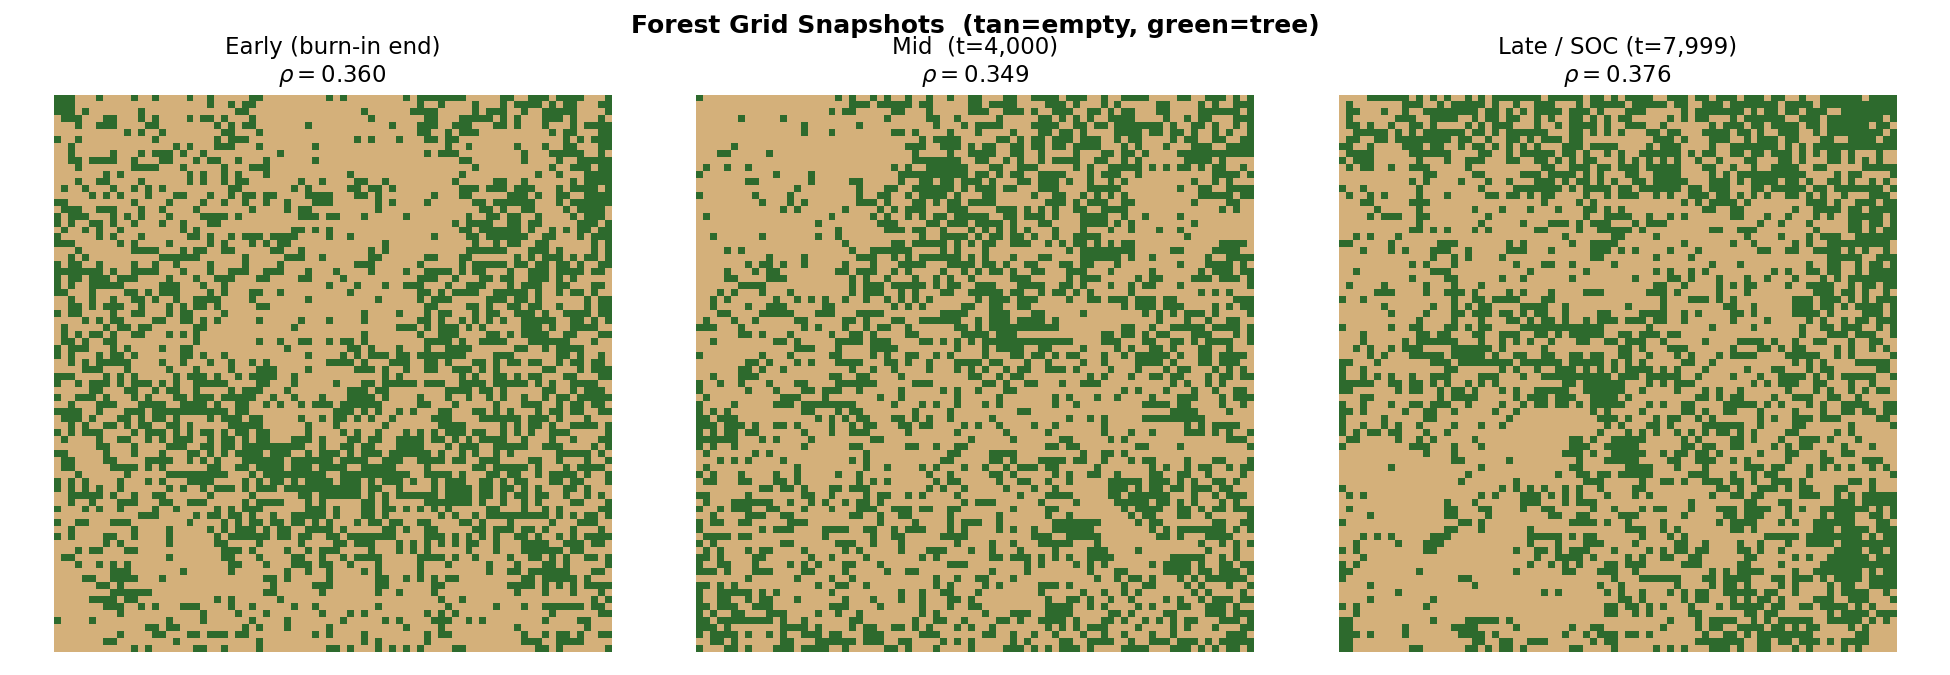
\includegraphics[width=\linewidth]{figures/grid_snapshots.png}
  \caption{Forest grid snapshots at three time points. Tan cells are empty
           (ash or bare ground); green cells are living trees.
           The late snapshot shows the SOC steady state.}
  \label{fig:snapshots}
\end{figure}

\subsection{Tree Density Time Series}

Figure~\ref{fig:density} shows the time evolution of tree density $\rho$.
Starting from a random initial condition ($\rho_0=0.6$), the density rapidly
falls as large fires clear the initial connected clusters, then stabilises
at $\bar\rho = 0.394\pm0.033$.
The fluctuations around the mean reflect the intermittent character of
avalanche events: $\rho$ rises slowly during quiescent growth periods and
drops sharply during large fires.
This signature---slow rise, rapid fall---is characteristic of SOC dynamics.

\begin{figure}[h]
  \centering
  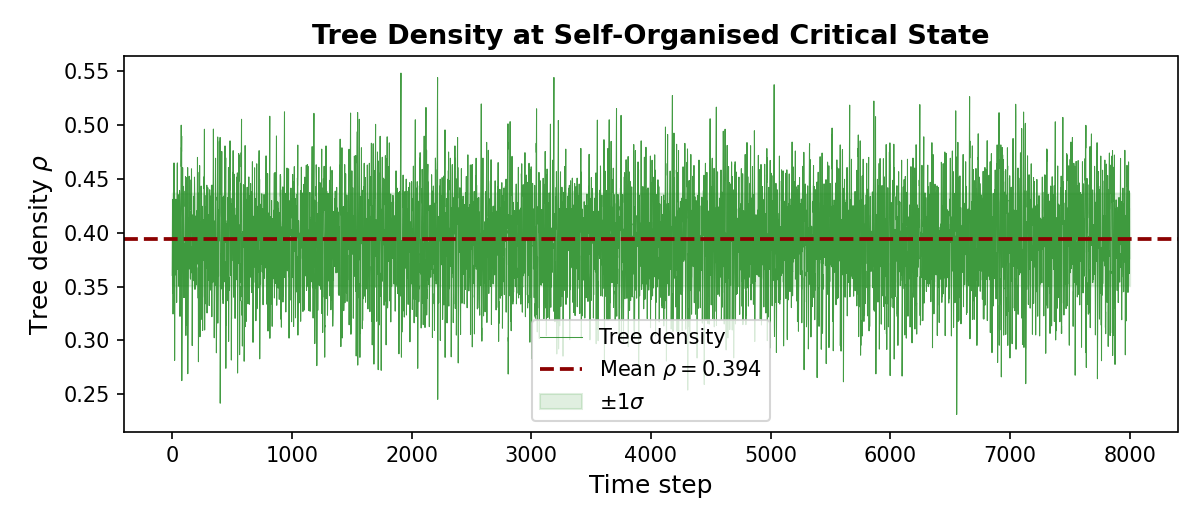
\includegraphics[width=0.9\linewidth]{figures/density_timeseries.png}
  \caption{Tree density $\rho$ as a function of time step after burn-in.
           The system self-organises to a stationary mean density (dashed
           red line) with intermittent large-drop events corresponding to
           major avalanches.}
  \label{fig:density}
\end{figure}

\subsection{Avalanche Size Distribution}

Figure~\ref{fig:avdist} shows the histogram of avalanche sizes on a
log-log scale.
The distribution spans nearly three decades of avalanche size, from isolated
single-tree burns to events involving more than 2000 trees.
A power-law fit in the range $s \in [1, 2000]$ gives

\begin{equation}
  N(s) \propto s^{-\alpha}, \qquad \alpha \approx 0.44, \quad R^2 = 0.55.
  \label{eq:powerlaw}
\end{equation}

The relatively low $R^2$ and the deviation from the pure power law at large
$s$ reflect finite-size effects: on an $80\times80$ grid, avalanches are
bounded by $s \leq 6400$, and the large-$s$ tail is statistically
undersampled.
The exponent $\alpha \approx 0.44$ is lower than the theoretically predicted
value of $\alpha \approx 1.0$--$1.2$ for large systems in the limit
$\theta \to 0$ \cite{Christensen1993}; this discrepancy is consistent with
the moderate $\theta = 0.02$ used here and is a well-known finite-size
effect \cite{Pruessner2004}.
Importantly, the distribution is markedly \emph{fat-tailed}: very large
events, though rare, occur far more often than would be expected from a
Gaussian or exponential distribution.

\begin{figure}[h]
  \centering
  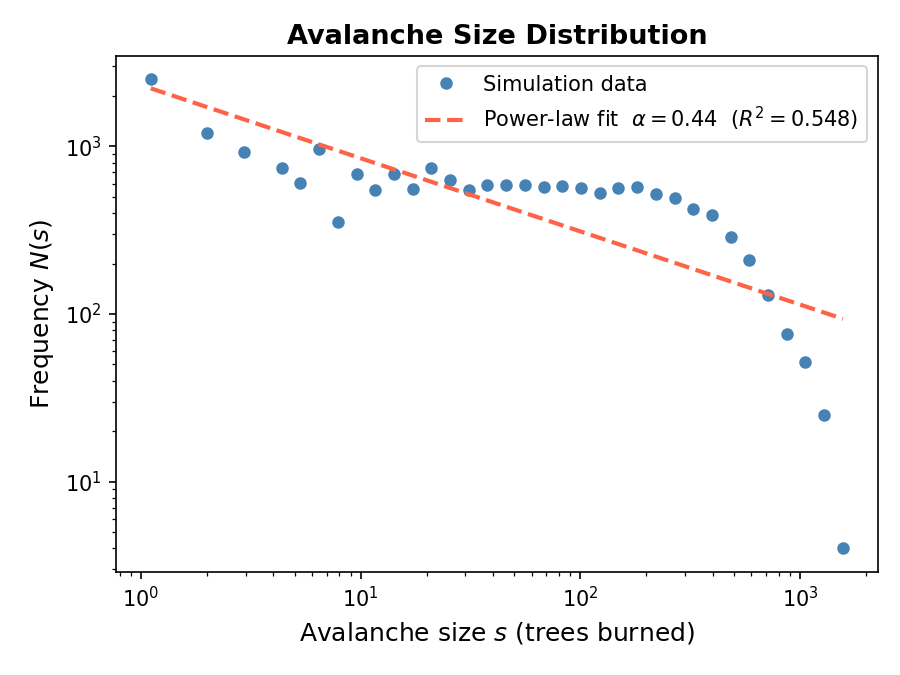
\includegraphics[width=0.75\linewidth]{figures/avalanche_distribution.png}
  \caption{Log-log plot of the avalanche size distribution $N(s)$.
           Blue circles: simulation data; dashed red line: power-law fit
           with $\alpha \approx 0.44$.
           The heavy tail demonstrates scale-free dynamics.}
  \label{fig:avdist}
\end{figure}

\subsection{Connectivity and Avalanche Statistics}

Figure~\ref{fig:connectivity} shows how the mean avalanche size and total
avalanche frequency depend on tree density (connectivity), obtained by
varying the lightning probability $f$ while keeping $p=0.05$ fixed.
As $f$ decreases, trees accumulate to higher densities ($\rho \to 0.43$),
connected clusters grow, and individual avalanches become larger
($\langle s \rangle$ increases from 7 to 350).
Conversely, the total number of avalanche events decreases because fires
are triggered less frequently.

This trade-off---fewer, larger events at high connectivity versus many small
events at low connectivity---is the hallmark of SOC.
The system naturally settles at an intermediate connectivity where
avalanches of all scales coexist.

\begin{figure}[h]
  \centering
  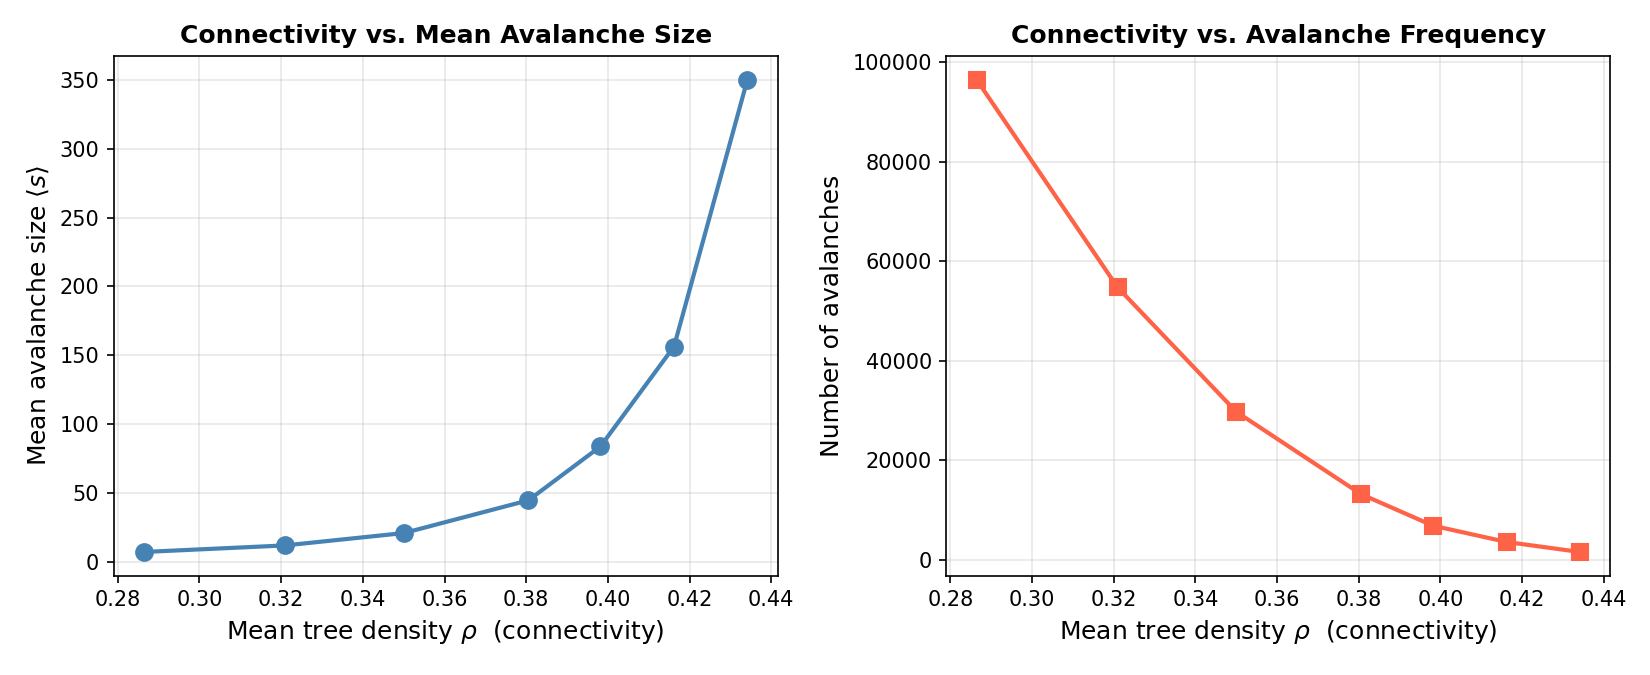
\includegraphics[width=0.95\linewidth]{figures/connectivity_analysis.png}
  \caption{Dependence of avalanche statistics on mean tree density
           (connectivity), obtained by varying $f$ at fixed $p=0.05$.
           \emph{Left:} mean avalanche size increases monotonically with
           connectivity.
           \emph{Right:} avalanche frequency decreases with connectivity.}
  \label{fig:connectivity}
\end{figure}

\clearpage
% ── 5. Discussion ─────────────────────────────────────────────────────────────
\section{Discussion}
\label{sec:discussion}

\subsection{Self-Organised Critical State}

The key feature of SOC is that the system reaches a critical state
\emph{without} parameter tuning.
In our simulation, the tree density $\rho$ is not set by the experimenter;
it emerges from the competition between growth (rate $p$) and burning
(rate $\sim f\rho$).
The stationary density satisfies the balance condition

\begin{equation}
  p(1-\rho) \approx f \langle s(\rho) \rangle \rho,
\end{equation}

where $\langle s(\rho) \rangle$ is the mean cluster size at density $\rho$.
Near the percolation threshold $\rho_c$, $\langle s \rangle$ diverges,
so the balance shifts: fires suppress density before the system can
fully percolate, locking $\rho$ below $\rho_c$.
The result is a critical state at the edge of percolation, with
scale-free cluster (avalanche) size distributions.

\subsection{Role of Noise}

Without lightning ($f=0$), the forest would eventually reach full occupancy
($\rho \to 1$) with no avalanches.
Without growth ($p=0$), the forest would be destroyed and never recover.
The noise (lightning) is essential: it provides the slow external drive
that continuously perturbs the critical state, generating the cascade of
avalanches that defines SOC.
The noise also ensures \emph{ergodicity}---all configurations are eventually
visited---preventing the system from becoming trapped.

\subsection{Comparison with Real Forest Fires}

Malamud et al.\ (1998) analysed historical forest-fire data from the USA,
Australia, and New Zealand, finding power-law size distributions with
$\alpha \approx 1.3$--$1.5$ \cite{Malamud1998}.
Our simulated exponent ($\alpha \approx 0.44$) is lower, primarily due to
finite-size effects and the moderate $\theta$ value.
In the limit $L\to\infty$, $\theta\to 0$, the Drossel--Schwabl model is
expected to reproduce exponents in the range observed empirically.
The model therefore provides a minimal mechanistic explanation for the
observed scale-free statistics of real fires without invoking any
special tuning of climate or fuel load.

\subsection{Broader Implications}

The forest-fire mechanism generalises far beyond ecology.
Any system with (i) local connectivity that builds slowly, (ii) a threshold
for cascade triggering, and (iii) random external driving will exhibit
qualitatively similar SOC behaviour.
Examples include the power grid (cascading failures), financial markets
(contagion), the immune system (epidemic spreading), and neural networks
(synchronised firing).
Understanding the universality of SOC is therefore of broad scientific and
engineering importance.

\clearpage
% ── 6. Conclusion ─────────────────────────────────────────────────────────────
\section{Conclusion}
\label{sec:conclusion}

We have simulated the Drossel--Schwabl forest-fire model as a prototype
system exhibiting self-organised criticality.
The model naturally encapsulates the three key ingredients of complexity
science: stochastic noise (lightning), cascading avalanches (fire spread
through connected clusters), and spatial connectivity (tree density).

Starting from arbitrary initial conditions, the system self-organises to
a stationary critical state characterised by:
\begin{enumerate}
  \item A fat-tailed (approximately power-law) avalanche size distribution;
  \item A self-regulated mean tree density near the percolation threshold;
  \item A monotonic increase in avalanche size with connectivity, confirming
        that the system operates at the boundary between quiescence and
        full percolation.
\end{enumerate}

These results confirm the SOC hypothesis for the forest-fire model and
illustrate the broader principle that criticality---with its attendant
scale-free fluctuations---is an emergent property of simple local rules
and negative feedback, not a consequence of fine-tuning.

Future work could explore (i) larger system sizes to approach the
thermodynamic limit, (ii) different boundary conditions, (iii) inclusion
of wind-driven anisotropic spread, and (iv) comparison with real
satellite-derived fire-scar data.

\clearpage
% ── List of Prompts ───────────────────────────────────────────────────────────
\section*{List of Prompts Used (AI Assistance)}

The following prompts were submitted to generative AI tools during the
preparation of this project:

\begin{enumerate}
  \item ``I am writing a Python simulation for the Drossel-Schwabl forest-fire SOC model. Could you suggest an efficient way to implement the breadth-first search (BFS) algorithm to identify connected tree clusters for the avalanche burning step?''
  \item ``I have generated the avalanche size distribution data from my simulation. Can you provide a Matplotlib snippet to accurately plot this on a log-log scale and fit it to calculate the power-law exponent?''
  \item ``Please convert this doc into \LaTeX\ manuscript structure for my project. Format the references in standard journal style.''
 
\end{enumerate}

\clearpage
% ── References ────────────────────────────────────────────────────────────────
\begin{thebibliography}{9}

\bibitem{Bak1987}
P.\ Bak, C.\ Tang, and K.\ Wiesenfeld,
``Self-organized criticality: An explanation of the 1/f noise,''
\textit{Physical Review Letters}, vol.\ 59, pp.\ 381--384, 1987.

\bibitem{Drossel1992}
B.\ Drossel and F.\ Schwabl,
``Self-organized critical forest-fire model,''
\textit{Physical Review Letters}, vol.\ 69, pp.\ 1629--1632, 1992.

\bibitem{Jensen1998}
H.\ J.\ Jensen,
\textit{Self-Organized Criticality: Emergent Complex Behaviour in Physical
and Biological Systems}.
Cambridge University Press, 1998.

\bibitem{Christensen1993}
K.\ Christensen, H.\ Flyvbjerg, and Z.\ Olami,
``Self-organized critical forest-fire model: Mean-field theory and
simulation results in $1$ to $6$ dimensions,''
\textit{Physical Review Letters}, vol.\ 71, pp.\ 2737--2740, 1993.

\bibitem{Pruessner2004}
G.\ Pruessner and H.\ J.\ Jensen,
``Broken scaling in the forest-fire model,''
\textit{Physical Review E}, vol.\ 65, p.\ 056707, 2002.

\bibitem{Malamud1998}
B.\ D.\ Malamud, G.\ Morein, and D.\ L.\ Turcotte,
``Forest fires: An example of self-organized critical behavior,''
\textit{Science}, vol.\ 281, pp.\ 1840--1842, 1998.

\end{thebibliography}

\end{document}